\section{Kategorie wzbogacone}\label{cat:sec:enriched}

Zamiast zbioru morfizmów pomiędzy dwoma obiektami rozważymy obiekt ustalonej kategorii monoidalnej. W ten sposób składanie może zachowywać strukturę liniową, porządek lub strukturę kategorii. Korzystamy z rozdziałów~\ref{cat:sec:monoidal} i~\ref{cat:sec:coherence}.

\subsection{Aksjomaty wzbogacenia}

Ustalmy lokalnie małą kategorię monoidalną $(\mathcal V,\otimes,I,\alpha,\lambda,\rho)$ (definicja~\ref{cat:def:monoidal}). Nie zakładamy symetrii.

\begin{definicja}[Kategoria wzbogacona]\label{cat:def:enriched-category}
$\mathcal V$-kategoria $\mathcal A$ składa się z klasy obiektów, obiektów $\mathcal A(X,Y)$ kategorii $\mathcal V$ dla każdej pary $X,Y$, morfizmów
\[
 m_{X,Y,Z}:\mathcal A(Y,Z)\otimes\mathcal A(X,Y)\to\mathcal A(X,Z)
\]
oraz jednostek $j_X:I\to\mathcal A(X,X)$. Pisząc $H_{XY}=\mathcal A(X,Y)$, wymagamy
\begin{equation}\label{cat:eq:enriched-assoc}
\begin{aligned}
&m_{W,X,Z}(m_{X,Y,Z}\otimes\id_{H_{WX}})\\
&=m_{W,Y,Z}(\id_{H_{YZ}}\otimes m_{W,X,Y})
  \alpha_{H_{YZ},H_{XY},H_{WX}},
\end{aligned}
\end{equation}
gdzie obie strony prowadzą z $(H_{YZ}\otimes H_{XY})\otimes H_{WX}$ do $H_{WZ}$, oraz
\begin{equation}\label{cat:eq:enriched-unit}
\begin{aligned}
 m_{X,Y,Y}(j_Y\otimes\id_{H_{XY}})&=\lambda_{H_{XY}},\\
 m_{X,X,Y}(\id_{H_{XY}}\otimes j_X)&=\rho_{H_{XY}}.
\end{aligned}
\end{equation}
Kategorię nazywamy małą, gdy jej obiekty tworzą zbiór.
\end{definicja}

Aksjomat łączności przedstawia diagram (pomijamy indeksy $m$):
\begin{center}
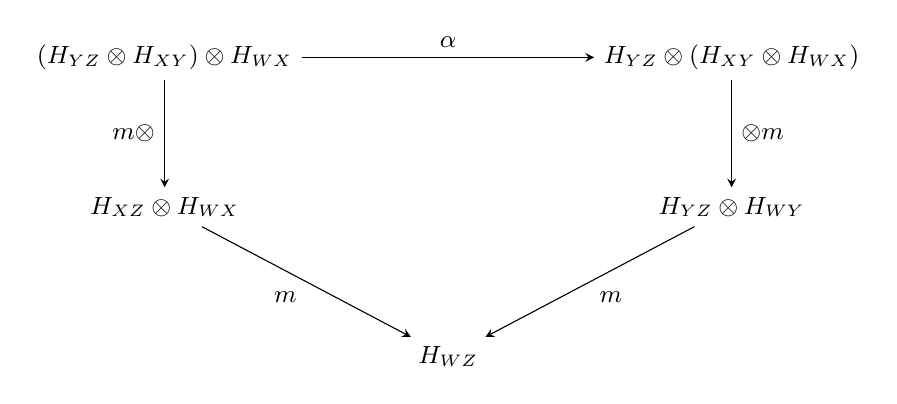
\begin{tikzpicture}[>=stealth,every node/.style={font=\small}]
 \node (a) at (0,3.8) {$(H_{YZ}\otimes H_{XY})\otimes H_{WX}$};
 \node (b) at (7.2,3.8) {$H_{YZ}\otimes(H_{XY}\otimes H_{WX})$};
 \node (c) at (0,1.9) {$H_{XZ}\otimes H_{WX}$};
 \node (d) at (7.2,1.9) {$H_{YZ}\otimes H_{WY}$};
 \node (e) at (3.6,0) {$H_{WZ}$};
 \draw[->] (a)--node[above] {$\alpha$} (b);
 \draw[->] (a)--node[left] {$m\otimes\id$} (c);
 \draw[->] (b)--node[right] {$\id\otimes m$} (d);
 \draw[->] (c)--node[below left] {$m$} (e);
 \draw[->] (d)--node[below right] {$m$} (e);
\end{tikzpicture}
\end{center}

\begin{twierdzenie}[Kategoria zwykła związana z kategorią wzbogaconą]\label{cat:thm:enriched-underlying}
$\mathcal V$-kategoria $\mathcal A$ wyznacza lokalnie małą kategorię zwykłą $\mathcal A_0$ o tych samych obiektach, w której
\[
 \Hom_{\mathcal A_0}(X,Y)=\Hom_{\mathcal V}(I,\mathcal A(X,Y)).
\]
Identyczności to $j_X$, a składanie dane jest wzorem
\[
 g\circ f=m_{X,Y,Z}(g\otimes f)\delta,\qquad
 \delta=\lambda_I^{-1}:I\to I\otimes I.
\]
\end{twierdzenie}
\begin{proof}
Lokalna małość $\mathcal V$ zapewnia istnienie wskazanych zbiorów morfizmów. Z lematu~\ref{cat:lem:unit-coherence} mamy $\lambda_I=\rho_I$. Z koherencji (twierdzenie~\ref{cat:thm:mac-lane-coherence}) wynika
\[
 \alpha_{I,I,I}(\delta\otimes\id_I)\delta
 =(\id_I\otimes\delta)\delta,
\]
gdyż obie strony są kanonicznymi morfizmami $I\to I\otimes(I\otimes I)$ zbudowanymi z izomorfizmów jednostkowych i łączności.

Dla $f:I\to\mathcal A(X,Y)$, $g:I\to\mathcal A(Y,Z)$, $h:I\to\mathcal A(Z,T)$ bifunktorialność daje
\[
 (h\circ g)\circ f
 =m_{X,Y,T}(m_{Y,Z,T}\otimes\id)
 ((h\otimes g)\otimes f)(\delta\otimes\id_I)\delta.
\]
Stosując~\eqref{cat:eq:enriched-assoc}, naturalność $\alpha$ i równość dla $\delta$, dostajemy
\[
 \begin{aligned}
 (h\circ g)\circ f
 &=m_{X,Z,T}(\id\otimes m_{X,Y,Z})
 (h\otimes(g\otimes f))(\id_I\otimes\delta)\delta\\
 &=h\circ(g\circ f).
 \end{aligned}
\]
Ostatnia równość wynika z bifunktorialności i definicji składania. Ponadto z~\eqref{cat:eq:enriched-unit} i naturalności izomorfizmów jednostkowych:
\[
\begin{aligned}
 j_Y\circ f&=\lambda_{\mathcal A(X,Y)}(\id_I\otimes f)\delta
 =f\lambda_I\delta=f,\\
 f\circ j_X&=\rho_{\mathcal A(X,Y)}(f\otimes\id_I)\delta
 =f\rho_I\delta=f.
\end{aligned}
\]
Otrzymujemy wszystkie aksjomaty kategorii.
\end{proof}

\subsection{Przykłady}

\begin{przyklad}[Zbiory]\label{cat:ex:enriched-set}
Dla $(\Set,\times,\{*\})$ wzbogacenie jest równoważne strukturze lokalnie małej kategorii zwykłej. Jednostki wskazują identyczności, a diagramy aksjomatów sprawdzone na elementach są dokładnie prawami zwykłego składania. Odwrotnie, zwykła kategoria wyznacza wszystkie wymagane dane, a funkcje zbiorów są wyznaczone przez wartości na elementach.
\end{przyklad}

\begin{przyklad}[Kategorie liniowe]\label{cat:ex:enriched-modules}
Dla przemiennego pierścienia $R$ z jedynką rozważamy kategorię unitarnych $R$-modułów z $\otimes_R$ i jednostką $R$ (twierdzenie~\ref{cat:thm:module-monoidal}). Własność uniwersalna iloczynu tensorowego identyfikuje morfizm składania z odwzorowaniem $R$-dwuliniowym na iloczynie kartezjańskim modułów. Jednostkę $j_X$ wyznacza $j_X(1)$, ponieważ $j_X(r)=rj_X(1)$. Na tensorach prostych aksjomaty są zwykłymi prawami łączności i jednostki. Odwrotnie, jeśli składanie dwuliniowe i identyczności spełniają te prawa, to liniowe morfizmy w diagramach są równe na generatorach (iterowanych tensorach prostych), więc są równe wszędzie. Dla $R=\mathbb Z$ otrzymujemy kategorie preaddytywne; nie wymaga się istnienia biproduktów ani obiektu zerowego.

Kategoria zwykła odzyskuje pierwotne morfizmy dzięki bijekcji $\Hom_R(R,M)\to M$, $f\mapsto f(1)$, której odwrotnością jest $x\mapsto(r\mapsto rx)$. Wzór składania obliczony na $1$ daje pierwotne składanie.
\end{przyklad}

\begin{przyklad}[Odległości Lawvere'a]\label{cat:ex:lawvere-metric}
Niech $\mathcal V$ będzie kategorią uporządkowaną $[0,\infty]$ z odwróconym porządkiem: morfizm $a\to b$ istnieje dokładnie wtedy, gdy $a\geq b$, i jest wtedy jedyny. Przyjmujemy $a\otimes b=a+b$ (z $a+\infty=\infty+a=\infty$), $I=0$. Dodawanie jest monotoniczne w obu argumentach, więc daje bifunktor; łączność i jednostkowość są ścisłe.

Wzbogacenie zbioru $X$ jest równoważne funkcji $d:X\times X\to[0,\infty]$ spełniającej
\[
 d(x,x)=0,\qquad d(x,z)\leq d(y,z)+d(x,y).
\]
Istnienie jednostki oznacza $0\geq d(x,x)$, a istnienie składania jest równoważne nierówności trójkąta. Równości morfizmów zachodzą automatycznie, bo pomiędzy ustalonymi obiektami istnieje co najwyżej jeden morfizm. Nie wymagamy symetrii, rozdzielania punktów ani skończoności odległości. W $\mathcal A_0$ istnieje morfizm $x\to y$ dokładnie wtedy, gdy $d(x,y)=0$. Dla zwykłej przestrzeni metrycznej $\mathcal A_0$ jest więc kategorią dyskretną i nie odzyskuje dodatnich odległości.
\end{przyklad}

\subsection{Funktory i transformacje naturalne wzbogacone}

\begin{definicja}[Funktor wzbogacony]\label{cat:def:enriched-functor}
Funktor wzbogacony $F:\mathcal A\to\mathcal B$ przypisuje obiektom obiekty, a parom $X,Y$ morfizmy
\[
 F_{XY}:\mathcal A(X,Y)\to\mathcal B(FX,FY)
\]
w $\mathcal V$ spełniające
\[
 F_{XX}j_X^{\mathcal A}=j_{FX}^{\mathcal B},\qquad
 F_{XZ}m^{\mathcal A}_{X,Y,Z}
 =m^{\mathcal B}_{FX,FY,FZ}(F_{YZ}\otimes F_{XY}).
\]
\end{definicja}

\begin{stwierdzenie}\label{cat:prop:enriched-functor-underlying}
Funktor wzbogacony wyznacza funktor $F_0:\mathcal A_0\to\mathcal B_0$ przez $F_0(f)=F_{XY}f$. Identyczności i składanie funktorów wzbogaconych definiujemy obiektowo i na składowych, a przyporządkowanie $F\mapsto F_0$ je zachowuje.
\end{stwierdzenie}
\begin{proof}
Aksjomat jednostki daje $F_0(j_X^{\mathcal A})=j_{FX}^{\mathcal B}$. Dla $f:I\to\mathcal A(X,Y)$ i $g:I\to\mathcal A(Y,Z)$
\[
 \begin{aligned}
 F_0(g\circ f)&=F_{XZ}m^{\mathcal A}_{X,Y,Z}(g\otimes f)\delta\\
 &=m^{\mathcal B}_{FX,FY,FZ}(F_{YZ}g\otimes F_{XY}f)\delta
 =F_0(g)\circ F_0(f).
 \end{aligned}
\]
Druga równość wynika z aksjomatu składania i bifunktorialności.

Dla $G:\mathcal B\to\mathcal D$ definiujemy $(GF)_{XY}=G_{FX,FY}F_{XY}$. Aksjomat jednostki dla złożenia wynika z $G_{FX,FX}F_{XX}j_X^{\mathcal A}=G_{FX,FX}j_{FX}^{\mathcal B}=j_{GFX}^{\mathcal D}$. Aksjomat składania wynika z kolejnych zastosowań aksjomatów $F,G$ i bifunktorialności:
\[
 (GF)_{XZ}m^{\mathcal A}
 =G_{FX,FZ}m^{\mathcal B}(F_{YZ}\otimes F_{XY})
 =m^{\mathcal D}((GF)_{YZ}\otimes(GF)_{XY}).
\]
Identyczności spełniają oba aksjomaty, ponieważ ich składowe są identycznościami w $\mathcal V$. Łączność i prawa jednostki wynikają z odpowiednich praw składania morfizmów w $\mathcal V$ oraz odwzorowań obiektów. Wreszcie $(GF)_0(f)=G_{FX,FY}F_{XY}f=G_0(F_0(f))$ i $(\id_{\mathcal A})_0=\id_{\mathcal A_0}$.
\end{proof}

\begin{przyklad}\label{cat:ex:enriched-functors}
W przypadku modułów funktory wzbogacone są funktorami liniowymi na zbiorach morfizmów: warunek składania można sprawdzać na tensorach prostych, a warunek jednostki na $1\in R$. Dla odległości Lawvere'a funktor wzbogacony istnieje dla zadanej funkcji $F$ dokładnie wtedy, gdy
\[
 d_{\mathcal B}(Fx,Fy)\leq d_{\mathcal A}(x,y)
\]
dla wszystkich $x,y$. Istnienie składowych jest równoważne tym nierównościom, a ich zgodność jest automatyczna z jednoznaczności morfizmów w kategorii uporządkowanej.
\end{przyklad}

\begin{definicja}[Transformacja naturalna wzbogacona]\label{cat:def:enriched-natural}
Dla funktorów wzbogaconych $F,G:\mathcal A\to\mathcal B$ transformacja naturalna wzbogacona $\eta:F\Rightarrow G$ to rodzina morfizmów $\eta_X:I\to\mathcal B(FX,GX)$ spełniająca
\begin{equation}\label{cat:eq:enriched-natural}
\begin{aligned}
 &m^{\mathcal B}_{FX,FY,GY}(\eta_Y\otimes F_{XY})
 \lambda_{\mathcal A(X,Y)}^{-1}\\
 &=m^{\mathcal B}_{FX,GX,GY}(G_{XY}\otimes\eta_X)
 \rho_{\mathcal A(X,Y)}^{-1}.
\end{aligned}
\end{equation}
Obie strony mają dziedzinę $\mathcal A(X,Y)$ i przeciwdziedzinę $\mathcal B(FX,GY)$.
\end{definicja}

\begin{stwierdzenie}\label{cat:prop:enriched-natural-underlying}
Transformacja naturalna wzbogacona $\eta$ wyznacza transformację naturalną zwykłą $F_0\Rightarrow G_0$ o składowych $\eta_X$.
\end{stwierdzenie}
\begin{proof}
Dla $f:I\to\mathcal A(X,Y)$ naturalność izomorfizmów jednostkowych daje
\[
 \lambda_{\mathcal A(X,Y)}^{-1}f=(\id_I\otimes f)\delta,\quad
 \rho_{\mathcal A(X,Y)}^{-1}f=(f\otimes\id_I)\delta.
\]
Składamy obie strony~\eqref{cat:eq:enriched-natural} z $f$. Bifunktorialność zamienia lewą stronę w $\eta_Y\circ F_0(f)$, a prawą w $G_0(f)\circ\eta_X$, na mocy wzoru składania w kategorii zwykłej. Otrzymujemy naturalność.
\end{proof}

\begin{uwaga}
Odwrotna implikacja wymaga dodatkowego założenia. Jeżeli $\Hom_{\mathcal V}(I,-)$ jest wierny, to zwykła naturalność danej rodziny $\eta_X$ implikuje wzbogaconą: dwa morfizmy w~\eqref{cat:eq:enriched-natural} są równe po złożeniu z każdym $f:I\to\mathcal A(X,Y)$, a z wierności wynika ich równość. Nie można zakładać tej wierności dla dowolnej kategorii monoidalnej.
\end{uwaga}


\subsection{Samowzbogacenie kategorii monoidalnie domkniętej}

Od tej chwili zakładamy, że $\mathcal V$ jest symetryczną kategorią monoidalnie domkniętą. Wewnętrzny obiekt Hom oznaczamy $[A,B]$, zgodnie z definicją~\ref{cat:def:monoidal-closed}. Ewaluację $\ev_{A,B}:[A,B]\otimes A\to B$ i jednoznaczność transpozycji przypomniano w stwierdzeniu~\ref{cat:prop:internal-hom-eval}.

W rachunkach z więcej niż dwoma czynnikami opuszczamy nawiasy i kanoniczne izomorfizmy jednostkowe. Jest to dozwolone przez twierdzenie~\ref{cat:thm:mac-lane-coherence}. Jeśli zmieniamy kolejność czynników, używamy symetrii $c_{A,B}:A\otimes B\to B\otimes A$; dla każdej zadanej permutacji jej kanoniczny morfizm jest jednoznaczny przez twierdzenie~\ref{cat:thm:symmetric-coherence}. W szczególności przestawienie dwóch czynników nie jest utożsamieniem obiektów na poziomie równości.

\begin{twierdzenie}[Samowzbogacenie]\label{cat:thm:self-enrichment}
Kategoria $\mathcal V$ ma kanoniczną strukturę $\mathcal V$-kategorii, oznaczaną $\underline{\mathcal V}$, z
\[
 \underline{\mathcal V}(A,B)=[A,B].
\]
Jej kategoria zwykła jest kanonicznie izomorficzna z $\mathcal V$.
\end{twierdzenie}
\begin{proof}
Definiujemy składanie $m:[B,C]\otimes[A,B]\to[A,C]$ jako transpozycję morfizmu
\[
 \begin{aligned}
 ([B,C]\otimes[A,B])\otimes A
 &\xrightarrow{\alpha}[B,C]\otimes([A,B]\otimes A)\\
 &\xrightarrow{\id\otimes\ev_{A,B}}[B,C]\otimes B
 \xrightarrow{\ev_{B,C}}C.
 \end{aligned}
\]
Jednostka $j_A:I\to[A,A]$ jest transpozycją $\lambda_A:I\otimes A\to A$.

Sprawdzimy łączność przez transpozycję odwrotną. Dwa morfizmy z $([C,D]\otimes[B,C])\otimes[A,B]$ do $[A,D]$ w aksjomacie łączności po dołączeniu czynnika $A$ i ewaluacji mają tę samą postać: najpierw ewaluacja $[A,B]\otimes A\to B$, następnie $[B,C]\otimes B\to C$, na końcu $[C,D]\otimes C\to D$. Dla drogi składającej najpierw $[C,D]$ z $[B,C]$ rozwijamy definicję ewaluacji złożenia, co daje dwie ostatnie ewaluacje. Dla drogi składającej najpierw $[B,C]$ z $[A,B]$ rozwinięcie daje dwie pierwsze. Przesunięcia nawiasów są kanoniczne, a przeniesienie ewaluacji przez nie wynika z naturalności $\alpha$. Jednoznaczność transpozycji daje łączność.

Dla lewej jednostki po transpozycji otrzymujemy na $(I\otimes[A,B])\otimes A$ najpierw ewaluację $[A,B]\otimes A$, następnie $\ev_{B,B}(j_B\otimes\id_B)=\lambda_B$. Jest to ta sama droga co $\ev_{A,B}(\lambda_{[A,B]}\otimes\id_A)$ przez naturalność $\lambda$ i koherencję. Dla prawej jednostki na $([A,B]\otimes I)\otimes A$ najpierw stosujemy $\ev_{A,A}(j_A\otimes\id_A)=\lambda_A$, następnie $\ev_{A,B}$. Równość z $\ev_{A,B}(\rho_{[A,B]}\otimes\id_A)$ wynika z aksjomatu trójkąta. Jednoznaczność transpozycji dowodzi obu praw jednostki.

Bijekcja
\[
 \Hom_{\mathcal V}(I,[A,B])\cong
 \Hom_{\mathcal V}(I\otimes A,B)\cong\Hom_{\mathcal V}(A,B)
\]
przypisuje $u$ morfizm $\ev_{A,B}(u\otimes\id_A)\lambda_A^{-1}$. Jednostce przypisuje $\id_A$. Dla dwóch elementów uogólnionych $u:I\to[A,B]$, $v:I\to[B,C]$ ewaluacja $m(v\otimes u)\delta$ na $A$ daje, po rozwinięciu definicji $m$ i użyciu naturalności jednostek, złożenie odpowiadających im morfizmów $A\to B$ i $B\to C$. Jawnie po wstawieniu $\delta$ do $I\otimes A$ dwa czynniki $I$ służą kolejno do ewaluacji $u$ i $v$; $\lambda_I\delta=\rho_I\delta=\id_I$ i trójkąt redukują ten morfizm do
\[
 \ev_{B,C}(v\otimes\id_B)\lambda_B^{-1}
 \ev_{A,B}(u\otimes\id_A)\lambda_A^{-1}.
\]
Bijekcje są więc zgodne ze składaniem. Na obiektach przyjmujemy identyczność, co daje izomorfizm kategorii zwykłych.
\end{proof}

\subsection{Wzbogacona kategoria funktorów}

Zakładamy dodatkowo, że $\mathcal V$ ma wszystkie małe iloczyny i equalizatory. Niech $\mathcal A$ będzie małą $\mathcal V$-kategorią, a $\mathcal B$ dowolną $\mathcal V$-kategorią. Małość $\mathcal A$ jest potrzebna do utworzenia poniższych iloczynów w $\mathcal V$.

\begin{definicja}[Rodzina naturalna z parametrem]\label{cat:def:parameter-natural}
Dla funktorów wzbogaconych $F,G:\mathcal A\to\mathcal B$ i obiektu $T\in\Ob(\mathcal V)$ rodzina $t_X:T\to\mathcal B(FX,GX)$ jest naturalna z parametrem $T$, jeśli dla wszystkich $X,Y$ dwa morfizmy z $T\otimes\mathcal A(X,Y)$ do $\mathcal B(FX,GY)$ są równe:
\[
 \begin{aligned}
 &m^{\mathcal B}(t_Y\otimes F_{XY}),\\
 &m^{\mathcal B}(G_{XY}\otimes t_X)c_{T,\mathcal A(X,Y)}.
 \end{aligned}
\]
Dla $T=I$, po złożeniu z $\lambda_{\mathcal A(X,Y)}^{-1}$, otrzymujemy warunek~\eqref{cat:eq:enriched-natural}, gdyż
$c_{I,H}\lambda_H^{-1}=\rho_H^{-1}$.
\end{definicja}

\begin{twierdzenie}[Obiekt naturalnych transformacji]\label{cat:thm:enriched-functor-hom}
Istnieje obiekt $E(F,G)$ kategorii $\mathcal V$ z morfizmami $p_X:E(F,G)\to\mathcal B(FX,GX)$ reprezentujący rodziny naturalne z parametrem: dla każdego $T$ istnieje naturalna bijekcja
\[
 \Hom_{\mathcal V}(T,E(F,G))
 \cong\{(t_X)_X:(t_X)_X\text{ jest naturalna z parametrem }T\}.
\]
Jest on equalizatorem
\begin{equation}\label{cat:eq:enriched-nat-equalizer}
 E(F,G)\longrightarrow
 \prod_X\mathcal B(FX,GX)
 \ \substack{\longrightarrow\\[-2pt]\longrightarrow}\
 \prod_{X,Y}[\mathcal A(X,Y),\mathcal B(FX,GY)].
\end{equation}
\end{twierdzenie}
\begin{proof}
Oznaczmy środkowy iloczyn przez $P$, a jego rzuty przez $q_X$. Dwa morfizmy z $P$ do prawego iloczynu określamy na składowych $(X,Y)$ przez transpozycje
\[
 m^{\mathcal B}(q_Y\otimes F_{XY}),\qquad
 m^{\mathcal B}(G_{XY}\otimes q_X)c_{P,\mathcal A(X,Y)}.
\]
Morfizm $t:T\to P$ wyrównuje obie strzałki wtedy i tylko wtedy, gdy wyrównuje wszystkie składowe, a przez naturalność transpozycji i symetrii jest to dokładnie warunek naturalności rodziny $t_X=q_Xt$. Własność iloczynu pozwala każdą taką rodzinę jednoznacznie złożyć do $P$, a własność equalizatora daje jej jedyną faktoryzację przez $E(F,G)$. Bijekcja jest naturalna w $T$, ponieważ dla $u:S\to T$ rodzina odpowiadająca złożeniu $tu$ ma składowe $t_Xu$. W przypadku pustej kategorii $\mathcal A$ oba iloczyny są końcowe i rodzina jest pusta; konstrukcja nadal działa.
\end{proof}

\begin{twierdzenie}[Wzbogacona kategoria funktorów]\label{cat:thm:enriched-functor-category}
Funktory wzbogacone $\mathcal A\to\mathcal B$ tworzą $\mathcal V$-kategorię $[\mathcal A,\mathcal B]_{\mathcal V}$, której obiektami Hom są $E(F,G)$. Jej kategoria zwykła ma jako morfizmy transformacje naturalne wzbogacone.
\end{twierdzenie}
\begin{proof}
Dla $F$ rodzina $j_{FX}^{\mathcal B}:I\to\mathcal B(FX,FX)$ jest naturalna z parametrem $I$, gdyż obie strony równania naturalności redukują się do $F_{XY}$ przez prawa jednostki. Wyznacza więc jednostkę $I\to E(F,F)$.

Niech $F,G,H$ będą funktorami. Oznaczmy rzuty z $E(G,H)$ przez $s_X$, a z $E(F,G)$ przez $t_X$. Kandydatem na rodzinę składania z parametrem $P=E(G,H)\otimes E(F,G)$ jest
\[
 u_X=m^{\mathcal B}(s_X\otimes t_X):P\to\mathcal B(FX,HX).
\]
Dowodzimy jej naturalności jako równości morfizmów na
$E(G,H)\otimes E(F,G)\otimes\mathcal A(X,Y)$.
Dla czytelności zapisujemy morfizm składania za pomocą kropki: np.\ $s_Y\cdot(t_Y\cdot F_{XY})$ oznacza złożenie morfizmów z trzech wskazanych czynników przez dwa morfizmy $m^{\mathcal B}$, a nie działanie na punktach obiektów $\mathcal V$. Jeżeli zmienia się kolejność czynników, przed tak zapisanym złożeniem stosujemy kanoniczną permutację dziedziny. Kolejno mamy
\[
 \begin{aligned}
 (s_Y\cdot t_Y)\cdot F_{XY}
 &=s_Y\cdot(t_Y\cdot F_{XY})\\
 &=s_Y\cdot(G_{XY}\cdot t_X)\\
 &=(s_Y\cdot G_{XY})\cdot t_X\\
 &=(H_{XY}\cdot s_X)\cdot t_X\\
 &=H_{XY}\cdot(s_X\cdot t_X).
 \end{aligned}
\]
Pierwsza, trzecia i ostatnia równość to aksjomaty łączności $\mathcal B$ złożone z odpowiednimi tensorami morfizmów. Druga korzysta z naturalności rodziny $t_X$ (przestawienie drugiego i trzeciego czynnika), a czwarta z naturalności $s_X$ (przestawienie pierwszego i trzeciego pierwotnego czynnika, które są teraz sąsiednie). Łącznie permutacja przenosi ostatni czynnik na początek, pozostawiając względny porządek dwóch pozostałych. Jest to właśnie $c_{P,\mathcal A(X,Y)}$ po kanonicznym nawiasowaniu, przez koherencję symetryczną. Otrzymaliśmy naturalność $u_X$.

Twierdzenie~\ref{cat:thm:enriched-functor-hom} daje jedyny morfizm $E(G,H)\otimes E(F,G)\to E(F,H)$ o tych składowych. Aby sprawdzić łączność, składamy obie drogi w aksjomacie łączności z rzutem na $\mathcal B(FX,KX)$ dla każdego $X$. Z definicji są to dwie drogi aksjomatu łączności $\mathcal B$, poprzedzone tensorami trzech rzutów i kanonicznymi izomorfizmami. Są równe z naturalności $\alpha$ i aksjomatu $\mathcal B$. Rzuty $p_X$ są wspólnie monomorficzne: równość wszystkich składowych daje równość po włączeniu equalizatora do iloczynu, a monomorficzność equalizatora daje równość morfizmów. Stąd łączność. Prawa jednostki sprawdzamy analogicznie po każdym rzucie, stosując odpowiednie prawo jednostki $\mathcal B$ oraz naturalność $\lambda,\rho$.

Dla parametru $I$ bijekcja z twierdzenia~\ref{cat:thm:enriched-functor-hom} identyfikuje morfizmy w kategorii zwykłej z transformacjami z definicji~\ref{cat:def:enriched-natural}. Jednostka ma składowe $j_{FX}$, a złożenie ma składowe będące złożeniami w $\mathcal B_0$: wynika to z poprzedniej konstrukcji, po dołączeniu $\delta:I\to I\otimes I$. Otrzymujemy zatem także zwykłą kategorię funktorów i transformacji wzbogaconych.
\end{proof}

\subsection{Wzbogacony lemat Yonedy}

Niech nadal $\mathcal A$ będzie mała, a $\mathcal V$ symetryczna monoidalnie domknięta z małymi iloczynami i equalizatorami. Dla $X\in\Ob(\mathcal A)$ definiujemy kowariantny funktor reprezentowalny $h^X:\mathcal A\to\underline{\mathcal V}$ przez $h^X(Y)=\mathcal A(X,Y)$. Jego działanie na obiektach Hom jest transpozycją
\[
 \mathcal A(Y,Z)\otimes\mathcal A(X,Y)
 \xrightarrow{m_{X,Y,Z}}\mathcal A(X,Z).
\]
Aksjomat jednostki funktora wynika po transpozycji odwrotnej z $m_{X,Y,Y}(j_Y\otimes\id)=\lambda$, a aksjomat składania z łączności $m$. Dokładniej, po dołączeniu $\mathcal A(X,Y)$ do dwóch obiektów Hom w aksjomacie składania obie drogi są odpowiednio składaniem najpierw dwóch morfizmów po lewej i najpierw dwóch po prawej; aksjomat~\eqref{cat:eq:enriched-assoc} daje ich równość, a jednoznaczność transpozycji przenosi ją na morfizmy do wewnętrznego Hom.

\begin{twierdzenie}[Wzbogacony lemat Yonedy, wersja kowariantna]\label{cat:thm:enriched-yoneda}
Dla funktora wzbogaconego $F:\mathcal A\to\underline{\mathcal V}$ istnieje izomorfizm w $\mathcal V$
\[
 [\mathcal A,\underline{\mathcal V}]_{\mathcal V}(h^X,F)\cong F(X),
\]
naturalny względem transformacji wzbogaconych $F\Rightarrow G$. W szczególności
\[
 \operatorname{Nat}_{\mathcal V}(h^X,F)
 \cong\Hom_{\mathcal V}(I,F(X)).
\]
\end{twierdzenie}
\begin{proof}
Oznaczmy przez $a_{YZ}:\mathcal A(Y,Z)\otimes F(Y)\to F(Z)$ transpozycję odwrotną składowej funktora $F_{YZ}$. Aksjomaty funktora i definicja samowzbogacenia dają
\[
 a_{YY}(j_Y\otimes\id)=\lambda_{F(Y)},\qquad
 a_{YT}(m_{Y,Z,T}\otimes\id)
 =a_{ZT}(\id\otimes a_{YZ})\alpha,
\]
gdzie w drugim równaniu dziedziną jest
$(\mathcal A(Z,T)\otimes\mathcal A(Y,Z))\otimes F(Y)$.
Równości te otrzymujemy przez transpozycję odwrotną aksjomatów funktora, ponieważ składanie wewnętrznego Hom zdefiniowano przez dwukrotną ewaluację.

Rodzina naturalna z parametrem $T$ od $h^X$ do $F$ jest, przez transpozycję składowych, rodziną
\[
 b_Y:T\otimes\mathcal A(X,Y)\to F(Y).
\]
Warunek naturalności jest równoważny następującej równości morfizmów z $T\otimes\mathcal A(Y,Z)\otimes\mathcal A(X,Y)$ do $F(Z)$ (z konwencją koherencji):
\begin{equation}\label{cat:eq:enriched-yoneda-naturality}
 b_Z(\id_T\otimes m_{X,Y,Z})
 =a_{YZ}(\id\otimes b_Y)(c_{T,\mathcal A(Y,Z)}\otimes\id).
\end{equation}
Istotnie, po transpozycji odwrotnej lewa strona warunku z definicji~\ref{cat:def:parameter-natural} najpierw stosuje działanie funktora $h^X$, czyli składanie $m$, i potem $b_Z$; prawa przestawia parametr $T$, stosuje $b_Y$ i następnie działanie $F$, czyli $a_{YZ}$. Obie transpozycje są bijekcjami.

Z takiej rodziny otrzymujemy morfizm
\[
 q=b_X(\id_T\otimes j_X)\rho_T^{-1}:T\to F(X).
\]
Odwrotnie, dla $q:T\to F(X)$ definiujemy
\[
 b_Y=a_{XY}(\id_{\mathcal A(X,Y)}\otimes q)c_{T,\mathcal A(X,Y)}.
\]
Aby sprawdzić~\eqref{cat:eq:enriched-yoneda-naturality}, w obu drogach przestawiamy $T$ na ostatnią pozycję w tensorze trzech czynników, korzystając z naturalności symetrii względem składania $m$ i koherencji. Po zastosowaniu $\id\otimes\id\otimes q$ lewa droga to $a_{XZ}(m_{X,Y,Z}\otimes\id)$, prawa to $a_{YZ}(\id\otimes a_{XY})\alpha$. Są równe z aksjomatu działania $F$. Zatem rodzina jest naturalna.

Zaczynając od $q$, po podstawieniu $Y=X$ i $j_X$ w powyższym wzorze, otrzymujemy ponownie $q$, gdyż naturalność symetrii oraz jej zgodność z jednostkami zamieniają $c_{T,\mathcal A(X,X)}(\id_T\otimes j_X)\rho_T^{-1}$ w $(j_X\otimes\id_T)\lambda_T^{-1}$. Aksjomat jednostki działania $F$ daje następnie $q$. Zaczynając od rodziny $b_Y$, stosujemy~\eqref{cat:eq:enriched-yoneda-naturality} dla pary $(X,Y)$ i podstawiamy $j_X$ w ostatnim czynniku $\mathcal A(X,X)$. Lewa strona po kanonicznym wstawieniu $I$ do dziedziny jest $b_Y$, ponieważ $m_{X,X,Y}(\id\otimes j_X)=\rho$. Prawa strona jest
$a_{XY}(\id\otimes q)c_{T,\mathcal A(X,Y)}$, z definicji $q$ i naturalności symetrii. Otrzymujemy więc pierwotną rodzinę.

Konstrukcje są naturalne w $T$: złożenie $q$ z $u:S\to T$ odpowiada rodzinie $b_Y(u\otimes\id)$, z bifunktorialności i naturalności symetrii. Z twierdzenia~\ref{cat:thm:enriched-functor-hom} dostajemy zatem naturalną bijekcję
\[
 \Hom_{\mathcal V}(T,E(h^X,F))\cong\Hom_{\mathcal V}(T,F(X)).
\]
Z lematu Yonedy w zwykłej kategorii $\mathcal V$ otrzymujemy żądany izomorfizm obiektów. Jego naturalność w $F$ wynika z tego, że dla transformacji wzbogaconej $\eta:F\Rightarrow G$ odpowiadającej rodzinie zwykłych morfizmów $\eta_Y:F(Y)\to G(Y)$, rodzina $b_Y$ przechodzi na $\eta_Yb_Y$, a jej ewaluacja na $j_X$ to $\eta_Xq$. Składowe $\eta_Y$ w tej postaci uzyskujemy przez izomorfizm z twierdzenia~\ref{cat:thm:self-enrichment}. Wybór $T=I$ daje ostatnią bijekcję z definicji kategorii zwykłej związanej z kategorią wzbogaconą.
\end{proof}

\begin{przyklad}[Liniowa wersja lematu Yonedy]\label{cat:ex:enriched-linear-yoneda}
Dla małej $R$-liniowej kategorii $\mathcal A$ oraz $R$-liniowego funktora $F$ do modułów izomorfizm z twierdzenia~\ref{cat:thm:enriched-yoneda} jest izomorfizmem $R$-modułów, a nie jedynie bijekcją zbiorów. Przypisuje transformacji $\eta$ element $\eta_X(\id_X)$, a elementowi $v\in F(X)$ rodzinę $\eta_Y(f)=F(f)(v)$ dla $f\in\mathcal A(X,Y)$. Liniowość w $f$ wynika z liniowości $F$ na zbiorach morfizmów, a naturalność z zachowywania składania. Wzory są wzajemnie odwrotne przez prawa jednostki i naturalność dla morfizmu $f:X\to Y$. Działania punktowe na rodzinach transformacji odpowiadają działaniom na $F(X)$, ponieważ każde $F(f)$ jest liniowe.
\end{przyklad}
